\chapter{Optimal transport}
\label{chap-ot}
\chapteroverview{Comparing two distributions requires a notion of the cost of moving mass between locations. Optimal transport turns that idea into an optimization problem. Starting with a small assignment problem, we introduce transport plans, explain when they coincide with maps, and use transport distances to compare colors, shapes, and texts.}

\section{Monge's problem}
In 1781, Gaspard Monge formulated the problem of moving earth from one place to another at minimum cost~\cite{Monge1781}. His cost was the distance traveled by each unit of mass. Other applications suggest other costs, such as travel time or the squared Euclidean distance.

\subsection{An assignment problem}
Consider six bakeries and six cafés in Paris. Each bakery supplies one batch of croissants, and each café requires one batch. In the assignment model, each batch goes to exactly one café, and each café receives exactly one batch. Both requirements matter: merely giving every bakery a destination would allow several bakeries to choose the same café.

Let $C_{ij}$ be the travel time from bakery $i$ to café $j$. The example in Figure~\ref{fig:image-cafe} has $C_{34}=10$. An admissible assignment is a permutation $\sigma$ of $\{1,\ldots,6\}$. For instance,
\begin{equation}\label{eq-bijection-exmp}
 (\sigma(1),\ldots,\sigma(6))=(5,2,6,1,3,4).
\end{equation}
Its total cost is
\begin{equation}\label{eq:cout}
 \operatorname{Cost}(\sigma)=\sum_{i=1}^6 C_{i,\sigma(i)}
 =10+7+15+10+14+9=65.
\end{equation}
This adds the six journey times. It does not model a single vehicle making a tour, nor the completion time of parallel deliveries.

\begin{figure}[htbp]\centering
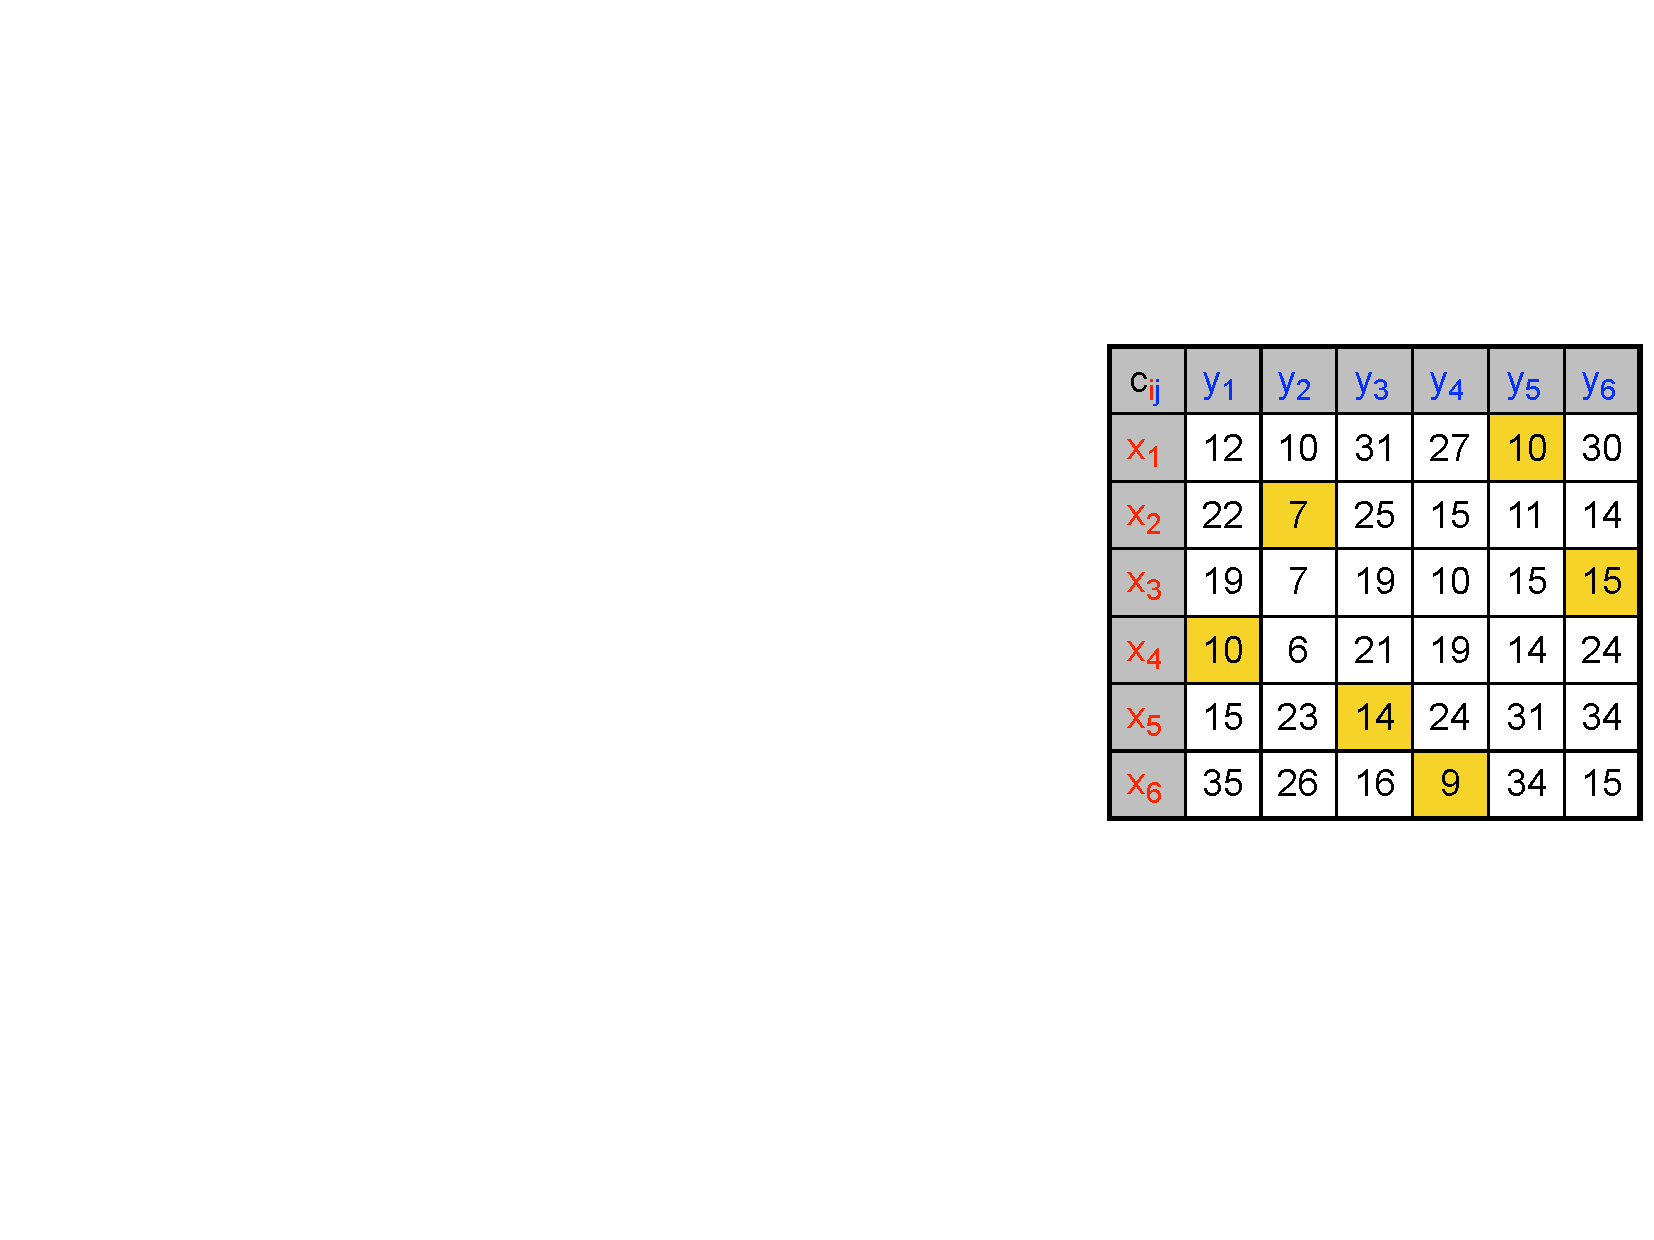
\includegraphics[width=.43\linewidth]{transport-hd/cafe-paris/map-paris-1-couts}\hfill
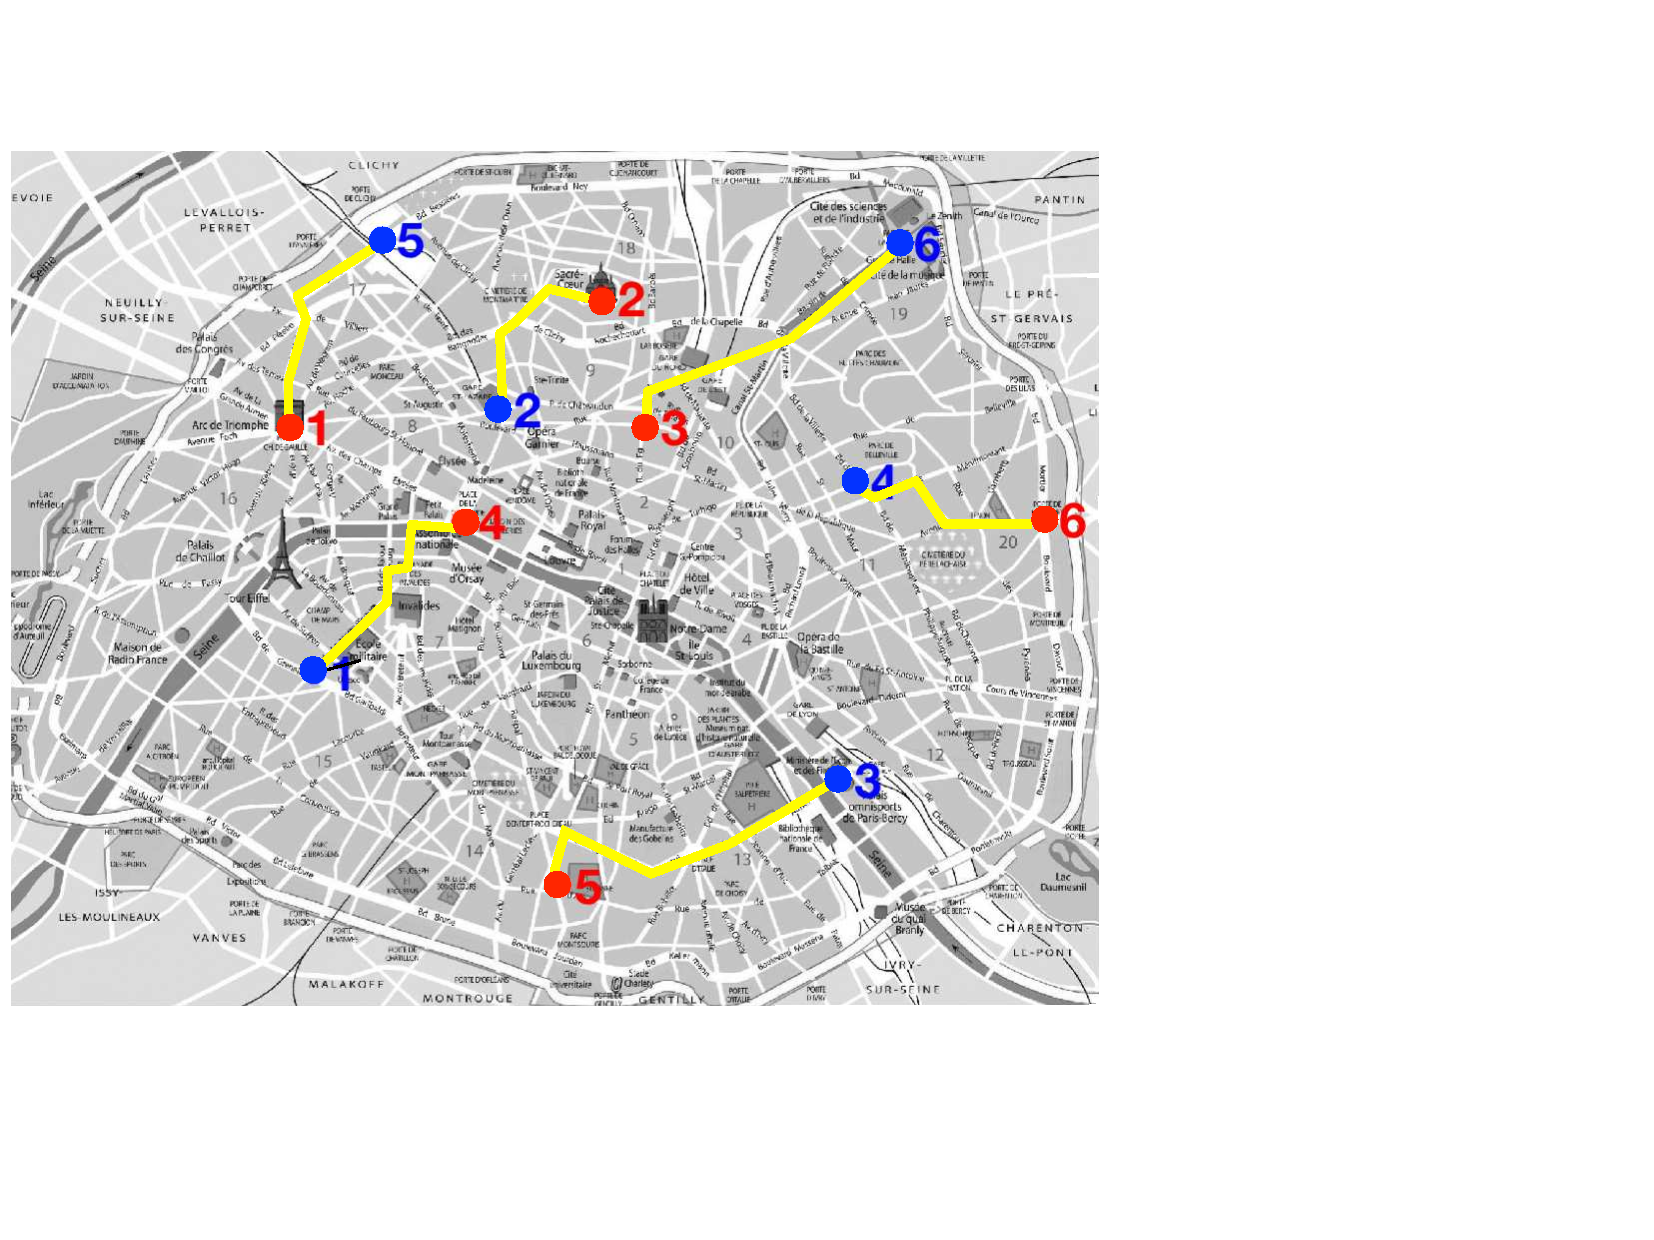
\includegraphics[width=.53\linewidth]{transport-hd/cafe-paris/map-paris-1}
\caption{Cost matrix and an assignment of the six bakeries (red) to the six cafés (blue). The highlighted entries give a total journey time of 65 minutes.}\label{fig:image-cafe}
\end{figure}

For $n$ equal batches on each side, the discrete Monge problem is
\begin{equation}\label{eq:monge}
 \min_{\sigma\in\Sigma_n}\sum_{i=1}^n C_{i,\sigma(i)},
\end{equation}
where $\Sigma_n$ is the set of permutations. In our example, the optimal value is 64, achieved by $(5,6,2,1,3,4)$. Exhaustively checking the $6!=720$ possibilities verifies this claim. There are $n!$ assignments in general, and $70!\approx1.198\times10^{100}$, so enumeration quickly becomes impractical.

\begin{figure}[htbp]\centering
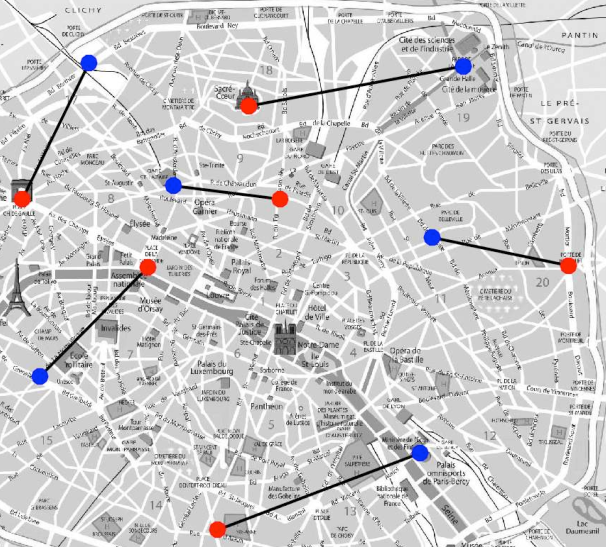
\includegraphics[width=.235\linewidth]{transport-hd/cafe-paris/ordre-croissant-64}\hfill
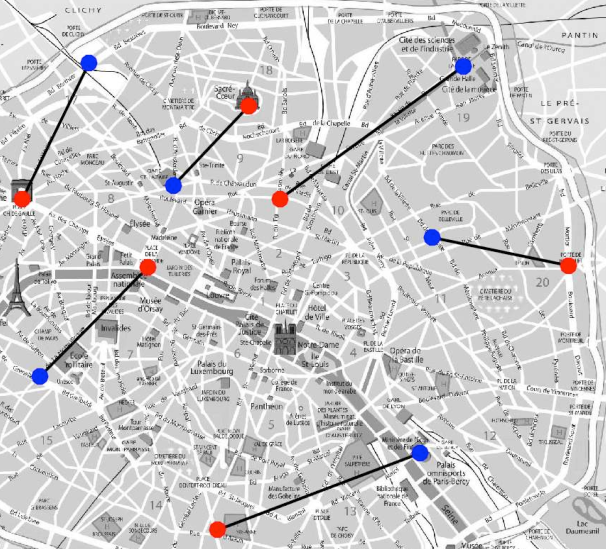
\includegraphics[width=.235\linewidth]{transport-hd/cafe-paris/ordre-croissant-65}\hfill
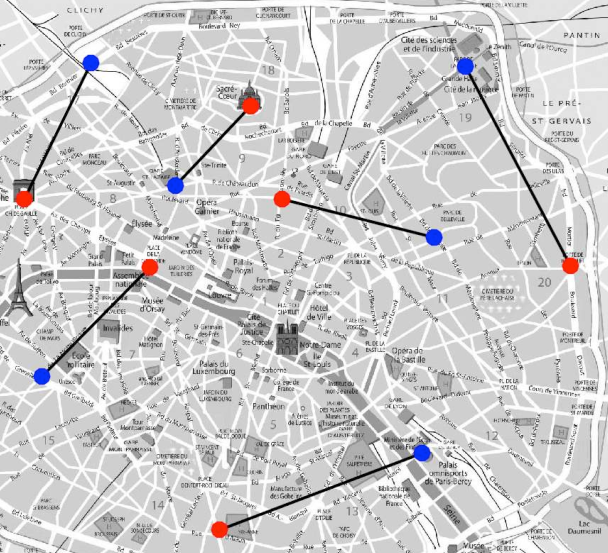
\includegraphics[width=.235\linewidth]{transport-hd/cafe-paris/ordre-croissant-66}\hfill
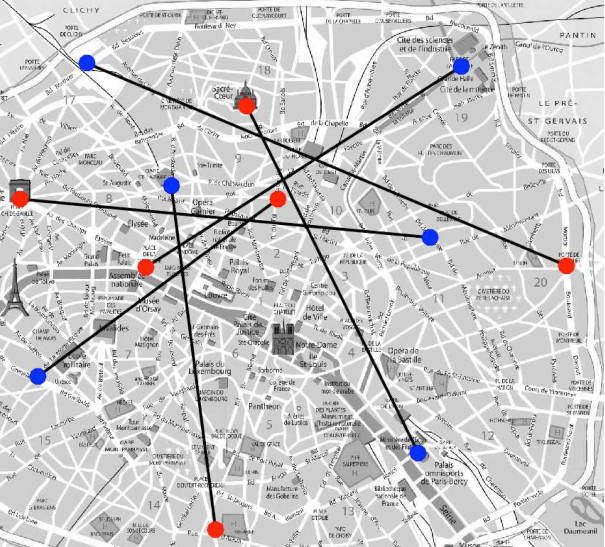
\includegraphics[width=.235\linewidth]{transport-hd/cafe-paris/ordre-croissant-152}
\caption{Four assignments with costs 64, 65, 66, and 152, from left to right.}\label{fig:order-increasing}
\end{figure}

\subsection{Sorting in one dimension}
Suppose the source locations $x_1\le\cdots\le x_n$ and target locations $y_1\le\cdots\le y_n$ lie on a line, with cost $C_{ij}=|x_i-y_j|$. Matching the points in sorted order is optimal. The key inequality is
\[
 |x-y|+|x'-y'|\le |x-y'|+|x'-y|
 \quad\text{when }x\le x'\text{ and }y\le y'.
\]
One can verify it by ordering the four points on the line. Whenever a permutation contains an inversion, swapping the two assigned targets does not increase the cost. Removing inversions successively produces the sorted matching. Equality can occur, so this optimal assignment need not be unique.

\begin{figure}[htbp]\centering
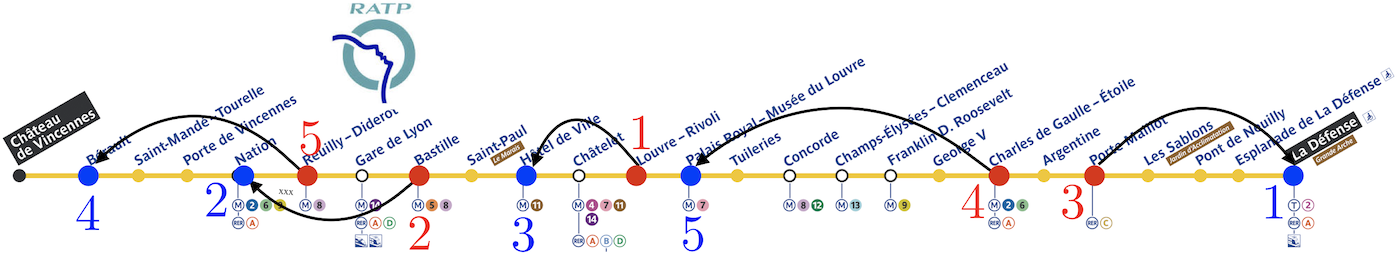
\includegraphics[width=.97\linewidth]{transport-hd/metro/plan-metro}
\caption{Sorted matching along a metro line, considered as a one-dimensional axis. For the indices shown, $\sigma:(1,2,3,4,5)\mapsto(3,2,1,5,4)$.}\label{fig:metro}
\end{figure}

The computational cost is therefore that of sorting the two lists. Insertion sort uses at most $n(n-1)/2$ comparisons per list, which is 2,415 for $n=70$. Merge sort reduces this to order $n\log n$. These are comparison counts for sorting, rather than estimates of every operation needed by a transport application.

In two dimensions there is no single ordering that solves the general problem. For the Euclidean distance cost, however, two segments in an optimal matching cannot cross transversely in their interiors. If segments $[x,y]$ and $[x',y']$ meet at $z$, the triangle inequality gives
\[
 |x-y'|+|x'-y|\le |x-z|+|z-y'|+|x'-z|+|z-y|
 =|x-y|+|x'-y'|.
\]
For a transverse crossing the inequality is strict, so exchanging destinations decreases the cost. Collinear overlaps or shared endpoints are degenerate cases and need not give a strict improvement. This observation does not suffice to compute an optimum: many noncrossing assignments can have different costs.

\begin{figure}[htbp]\centering
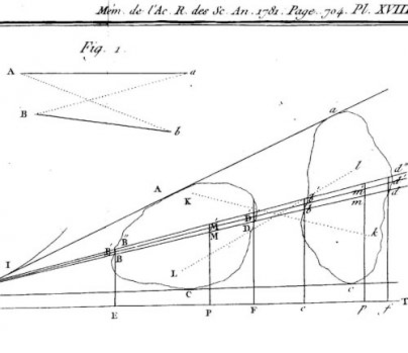
\includegraphics[width=.30\linewidth]{transport-hd/monge-2d/article-monge}\hfill
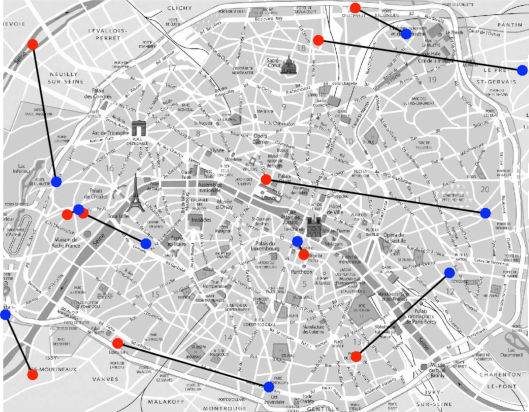
\includegraphics[width=.30\linewidth]{transport-hd/monge-2d/example-10}\hfill
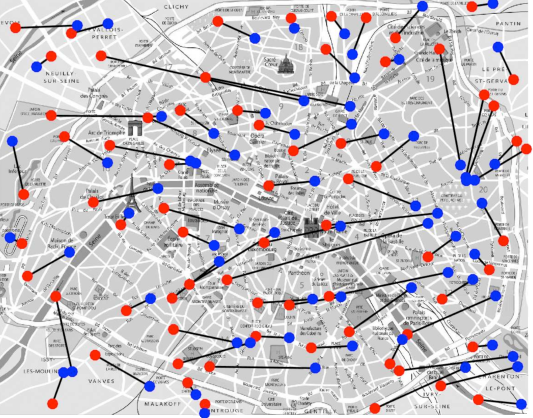
\includegraphics[width=.30\linewidth]{transport-hd/monge-2d/example-70}
\caption{An illustration from Monge’s original article~\cite{Monge1781} and two optimal Euclidean matchings in the plane.}\label{fig:ot2d}
\end{figure}

\section{Kantorovich's relaxation}
\label{sec-kanto}
Kantorovich's formulation allows mass to split between destinations~\cite{Kantorovich42}. It replaces discrete choices by nonnegative quantities subject to linear conservation constraints, making optimal transport a linear programming problem.

\subsection{From permutations to matrices}
Represent a permutation by $P_{ij}=1$ when $j=\sigma(i)$ and $P_{ij}=0$ otherwise. For example, the permutations $(1,2,3)$, $(3,2,1)$, and $(2,1,3)$ correspond to
\[
 \begin{pmatrix}1&0&0\\0&1&0\\0&0&1\end{pmatrix},\qquad
 \begin{pmatrix}0&0&1\\0&1&0\\1&0&0\end{pmatrix},\qquad
 \begin{pmatrix}0&1&0\\1&0&0\\0&0&1\end{pmatrix}.
\]
Each row and each column sums to one. If $\mathcal P_n$ denotes this set of permutation matrices, then~\eqref{eq:monge} is equivalent to
\begin{equation}\label{eq:mongematrix}
 \min_{P\in\mathcal P_n}\langle C,P\rangle,
 \qquad \langle C,P\rangle=\sum_{i,j}C_{ij}P_{ij}.
\end{equation}
Relaxing the binary constraint gives the doubly stochastic matrices
\begin{equation}\label{eq:bistoch}
 \mathcal B_n=\left\{P\in\RR_+^{n\times n}:\sum_jP_{ij}=1,\ \sum_iP_{ij}=1\right\}.
\end{equation}
Nonnegativity and the row sums already imply $P_{ij}\le1$. The relaxed problem is
\begin{equation}\label{eq:kantoassign}
 \min_{P\in\mathcal B_n}\langle C,P\rangle.
\end{equation}
The set $\mathcal B_n$ is compact and convex: for $P,Q\in\mathcal B_n$ and $0\le t\le1$, the matrix $(1-t)P+tQ$ is still feasible. A minimizer exists because the objective is continuous.

The development of linear programming, including Dantzig's simplex method~\cite{Dantzig51}, made these problems computationally accessible. Specialized assignment algorithms, such as implementations of the Hungarian method, solve the dense $n\times n$ assignment problem in $O(n^3)$ operations. This bound should not be attributed to the general simplex method, whose worst-case running time is not polynomial.

\subsection{Why the relaxation is exact for equal masses}
The Birkhoff--von Neumann theorem states that every doubly stochastic matrix is a convex combination of permutation matrices~\cite{birkhoff,von1953certain}:
\[
 P=\sum_{k=1}^K\lambda_k P^{(k)},
 \qquad \lambda_k\ge0,\quad\sum_k\lambda_k=1.
\]
Consequently, $\langle C,P\rangle=\sum_k\lambda_k\langle C,P^{(k)}\rangle$ cannot be smaller than the least permutation cost. Since every permutation matrix is feasible for the relaxation, we obtain
\begin{equation}\label{eq:monge-vs-kanto}
 \min_{P\in\mathcal B_n}\langle C,P\rangle
 =\min_{P\in\mathcal P_n}\langle C,P\rangle.
\end{equation}
Thus at least one optimal plan is a permutation. It does not follow that every optimal plan is a permutation: the average of two distinct optimal permutations is also optimal. If all costs vanish, every doubly stochastic matrix is optimal.

A useful way to certify an optimal value is to find numbers $u_i,v_j$ satisfying $u_i+v_j\le C_{ij}$. Every $P\in\mathcal B_n$ then satisfies
\[
 \langle C,P\rangle\ge\sum_{i,j}(u_i+v_j)P_{ij}=\sum_i u_i+\sum_jv_j.
\]
For the Paris example, $u=(2,3,3,0,5,2)$ and $v=(10,4,9,7,8,11)$ satisfy all 36 inequalities and their entries sum to 64. Together with an assignment of cost 64, they prove optimality without listing all permutations.

\subsection{Different numbers of points and unequal masses}
Now let $n$ bakeries supply amounts $a_i\ge0$, and let $m$ cafés require amounts $b_j\ge0$, with common total mass
\[
 \sum_{i=1}^n a_i=\sum_{j=1}^m b_j=s.
\]
A transport plan belongs to
\[
 \mathcal B(a,b)=\left\{P\in\RR_+^{n\times m}:\sum_jP_{ij}=a_i,\ \sum_iP_{ij}=b_j\right\}.
\]
When $s>0$, the plan $P_{ij}=a_i b_j/s$ proves feasibility. When $s=0$, the only plan is zero. The transport problem is
\begin{equation}\label{eq-kanto-gen}
 \min_{P\in\mathcal B(a,b)}\sum_{i=1}^n\sum_{j=1}^m C_{ij}P_{ij}.
\end{equation}
For finite costs, compactness again ensures the existence of a minimizer. An entry $P_{ij}$ is the amount shipped from $i$ to $j$, and $C_{ij}$ is its cost per unit of mass.

\begin{figure}[htbp]\centering
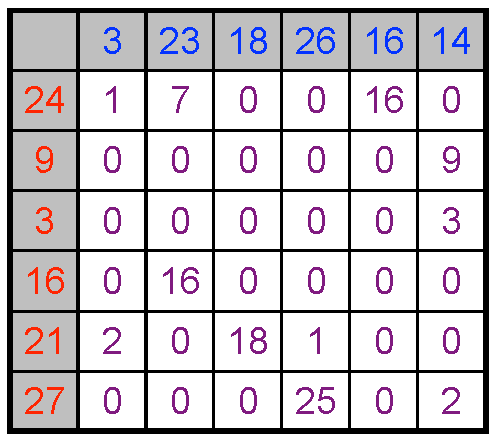
\includegraphics[width=.235\linewidth]{transport-hd/kantorovitch/coupling-array}\hfill
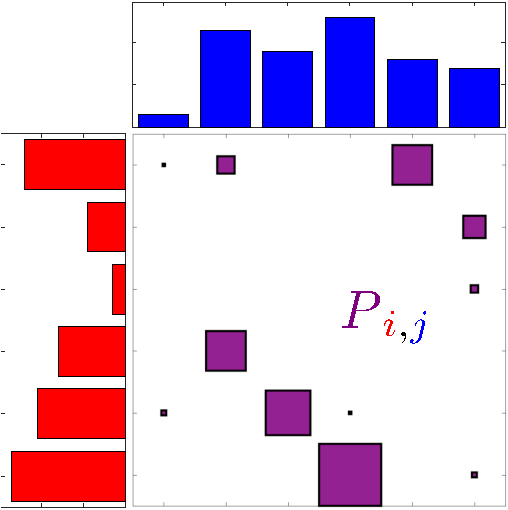
\includegraphics[width=.235\linewidth]{transport-hd/kantorovitch/coupling-squares}\hfill
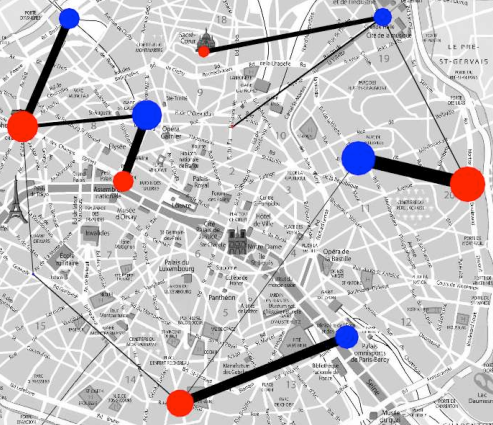
\includegraphics[width=.235\linewidth]{transport-hd/kantorovitch/coupling-map}\hfill
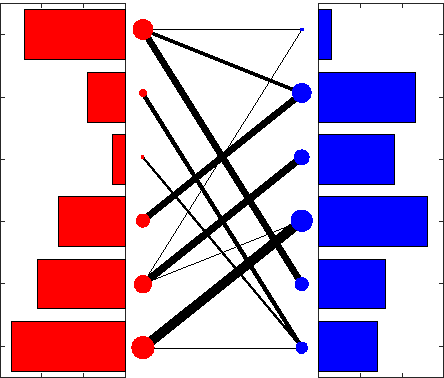
\includegraphics[width=.235\linewidth]{transport-hd/kantorovitch/coupling-bipartite}
\caption{Four views of the same coupling: its matrix entries, a display of their magnitudes by squares, weighted segments in space, and a bipartite graph. Row and column sums give the prescribed masses $a$ and $b$.}\label{fig:coupling-visu}
\end{figure}

Mass splitting can now be necessary. One bakery with mass 2 and two cafés requiring mass 1 each have the unique feasible plan $P=(1\;1)$. A map that sends the entire source mass to a single target cannot realize these marginals. This explains why a transport plan is more general than a transport map. In the equal-mass case $a_i=b_j=1$, we recover $\mathcal B_n$; for probability masses $a_i=b_j=1/n$, the corresponding plans are $P/n$.

\section{Measures and transport distances}
The same ideas apply to probability measures, including discrete distributions $\mu=\sum_i a_i\delta_{x_i}$ and $\nu=\sum_jb_j\delta_{y_j}$. A coupling $\pi\in\Pi(\mu,\nu)$ is a probability measure on pairs $(x,y)$ with marginals $\mu$ and $\nu$. A measurable map $T$ induces a coupling $(\mathrm{Id},T)_\#\mu$ when $T_\#\mu=\nu$; the notation means that applying $T$ to a random variable of law $\mu$ gives one of law $\nu$.

For probability measures on $\RR^d$ with finite second moments, the quadratic transport distance is
\begin{equation}\label{eq-wasserstein}
 W_2(\mu,\nu)^2=\min_{\pi\in\Pi(\mu,\nu)}\int |x-y|^2\,\d\pi(x,y).
\end{equation}
In the discrete case, this is~\eqref{eq-kanto-gen} with $C_{ij}=|x_i-y_j|^2$. The distance depends on both masses and locations: equal weight vectors at different locations need not describe the same measure. The square root $W_2$ is a metric, and $W_2(\mu,\nu)=0$ exactly when $\mu=\nu$. Its square generally fails the triangle inequality; for point masses at 0, 1, and 2, the relevant squared distances are 1, 1, and 4.

Brenier's theorem gives a precise condition under which the optimal coupling is a map~\cite{Brenier91}. If the source $\mu$ is absolutely continuous with respect to Lebesgue measure and both measures have finite second moments, the quadratic problem has a unique optimal coupling. It is induced by a map $T=\nabla\varphi$, where $\varphi$ is convex, and $T$ is unique $\mu$-almost everywhere. Absolute continuity and the choice of cost matter; one cannot assert this conclusion for arbitrary measures and arbitrary costs.

\section{Applications}
\subsection{Transferring a color palette}
For two images with the same number $n$ of pixels, let $x_i,y_j\in\RR^3$ be their RGB colors. An assignment minimizing $\sum_i|x_i-y_{\sigma(i)}|^2$ gives an output whose color at source position $i$ is $y_{\sigma(i)}$. Every target color is used once, so the output has exactly the target's empirical color distribution. The optimization limits changes in color, but contains no spatial regularity term; preservation of edges and textures is therefore not guaranteed.

\begin{figure}[htbp]\centering
\begin{tabular}{@{}ccc@{}}
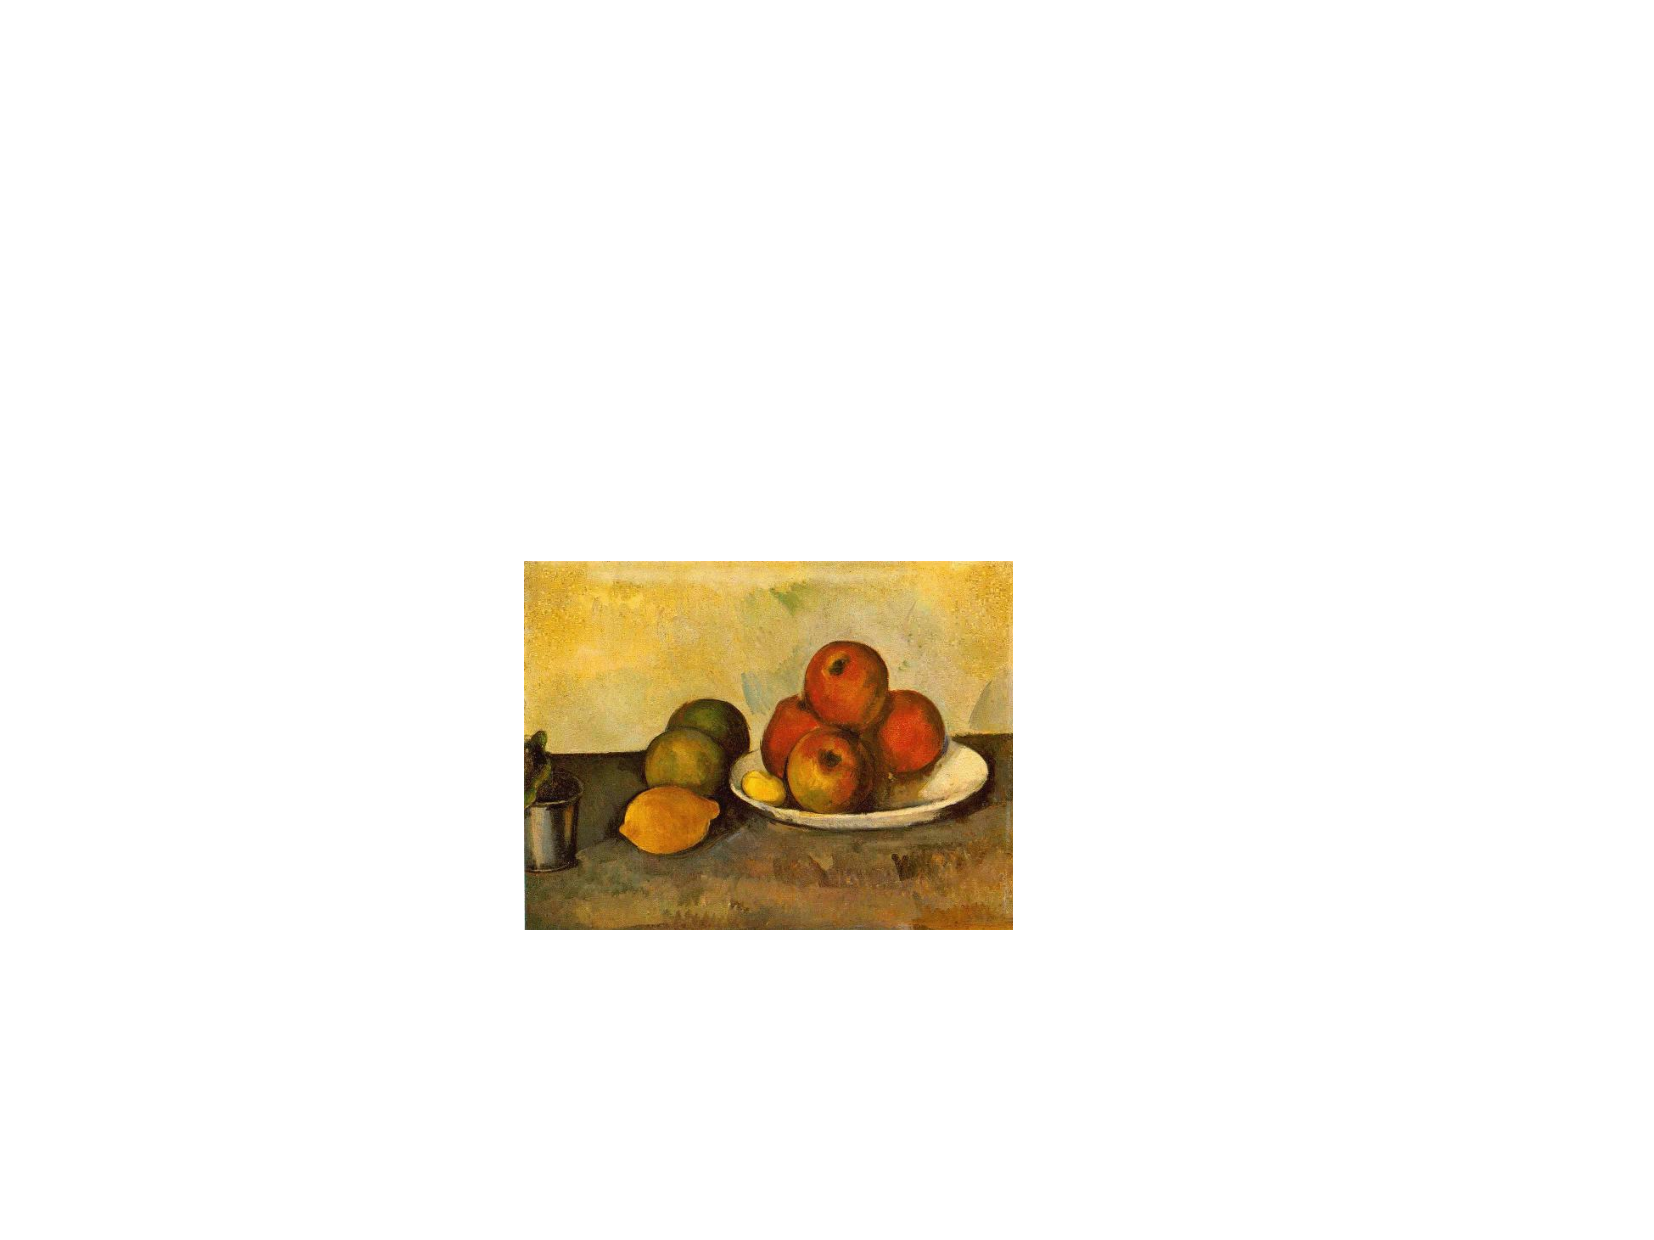
\includegraphics[width=.29\linewidth]{transport-hd/applis/painting-2} &
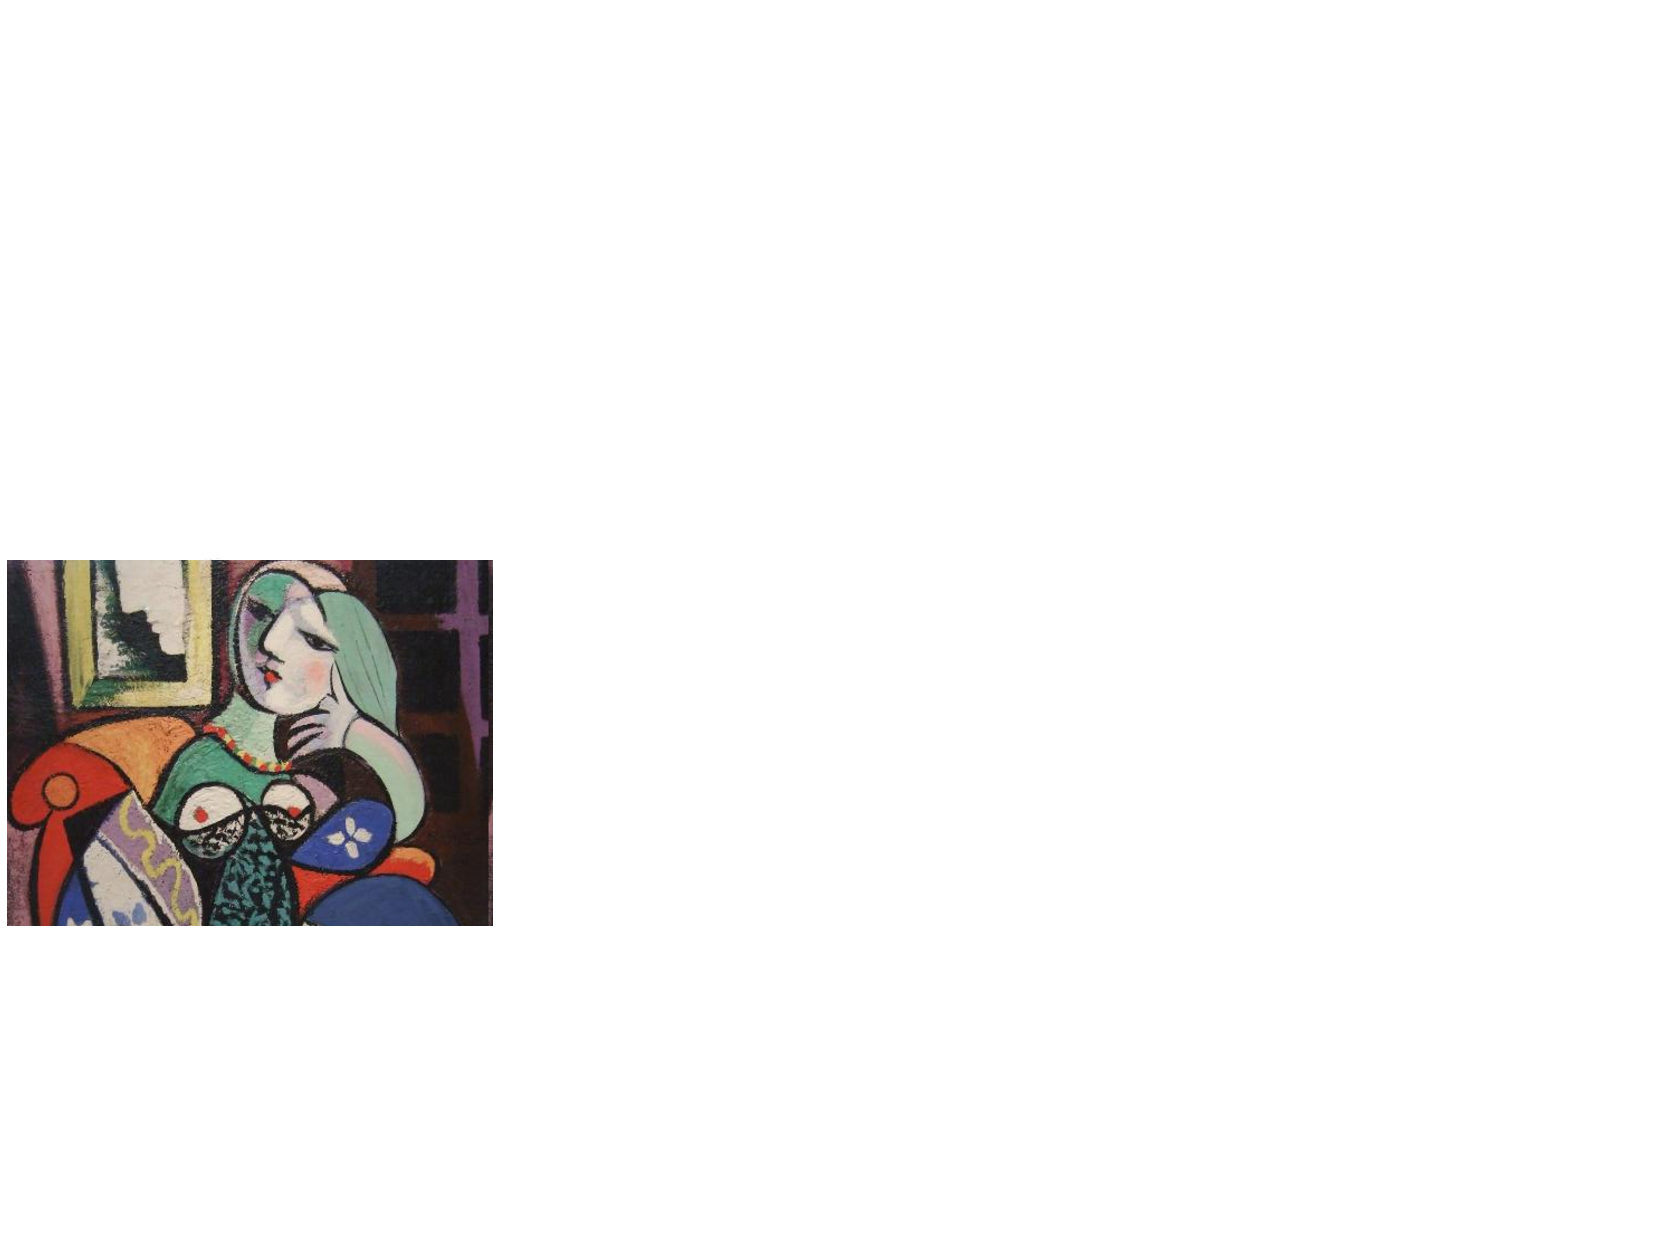
\includegraphics[width=.29\linewidth]{transport-hd/applis/painting-1} &
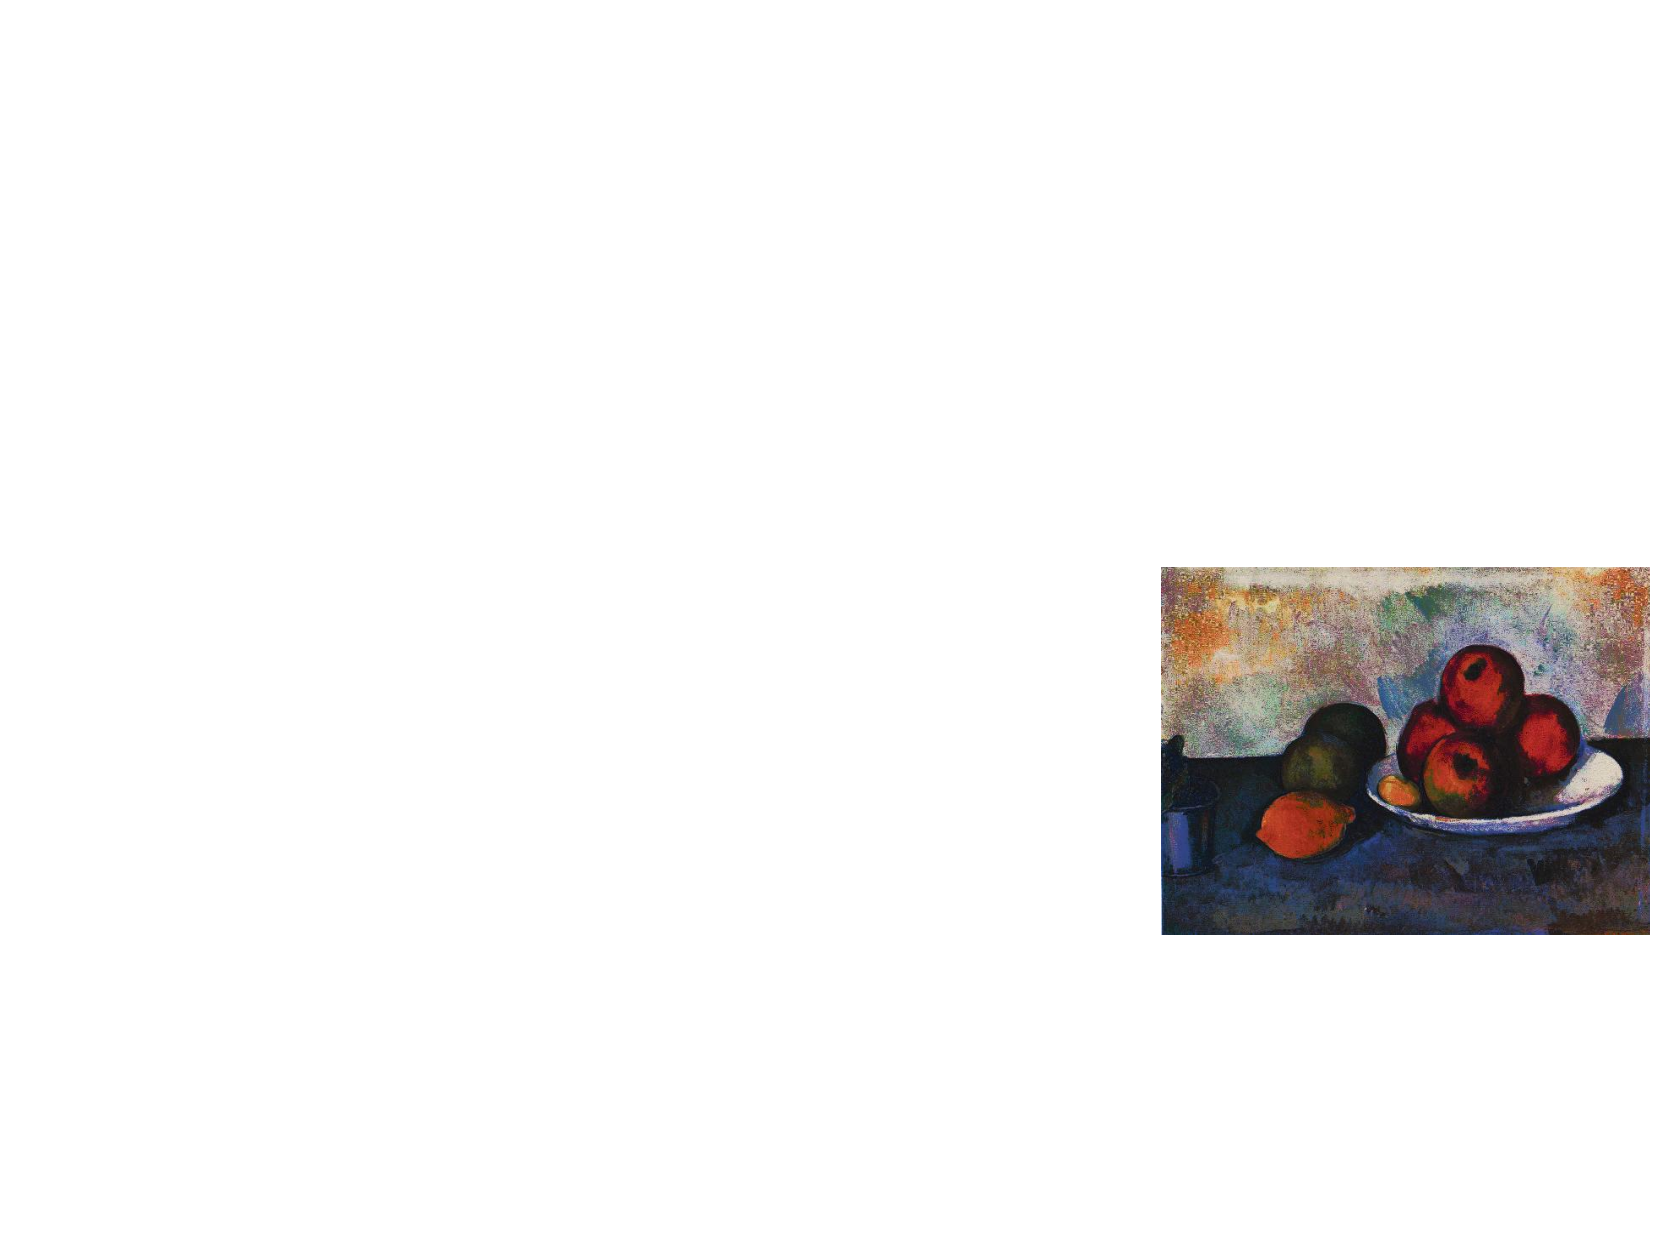
\includegraphics[width=.29\linewidth]{transport-hd/applis/painting-2-equalized}\\[3pt]
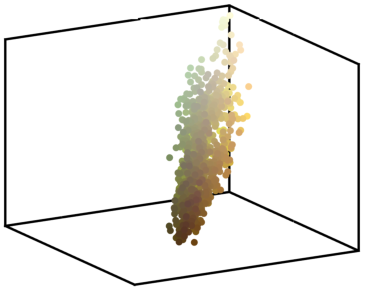
\includegraphics[width=.29\linewidth]{transport-hd/applis/painting-2-histo} &
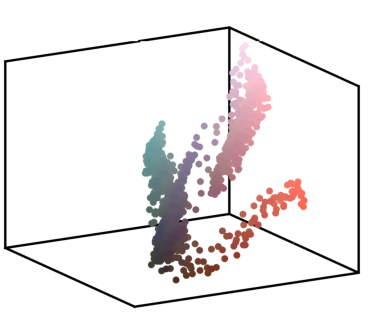
\includegraphics[width=.29\linewidth]{transport-hd/applis/painting-1-histo} &
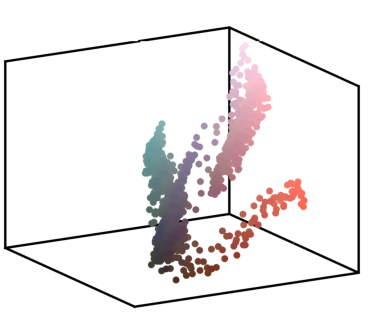
\includegraphics[width=.29\linewidth]{transport-hd/applis/painting-1-histo}
\end{tabular}
\caption{Color-palette transfer. Columns: source, target, and recolored source. Top: colors on the image grid; bottom: the corresponding point clouds in RGB space. A permutation of the target colors gives the same color cloud in the last two columns.}\label{fig:image-eq}
\end{figure}

This distinction separates color transport from moving pixels in the image plane. Here the locations being transported are points in color space; the display grid stays fixed. With different image sizes or weighted color clusters, one uses a coupling and a specified rule to convert that coupling into output colors. A barycentric average of coupled colors need not preserve the target histogram exactly.

\subsection{Barycenters of shapes}
The Euclidean weighted mean of three points minimizes $\alpha|x-r|^2+\beta|y-r|^2+\gamma|z-r|^2$, where $\alpha,\beta,\gamma\ge0$ and $\alpha+\beta+\gamma=1$. Its value is $r=\alpha x+\beta y+\gamma z$. Replacing squared Euclidean distances by squared transport distances defines a Wasserstein barycenter~\cite{agueh2011barycenters}:
\begin{equation}\label{eq-bary}
 \min_{\rho\in\mathcal P_2(\RR^d)}
 \alpha W_2(\mu,\rho)^2+\beta W_2(\nu,\rho)^2+\gamma W_2(\eta,\rho)^2.
\end{equation}
Here $\mathcal P_2$ is the set of probability measures with finite second moment. In a grid-based computation, one instead restricts $\rho$ to probability weights on that grid. A shape can be represented by a uniform density inside it, normalized to total mass one. Changing the three weights produces a family of interpolated distributions (Figure~\ref{fig:barycenters}). These distributions need not themselves be uniform inside a sharp shape, and uniqueness requires additional assumptions.

\begin{figure}[htbp]\centering
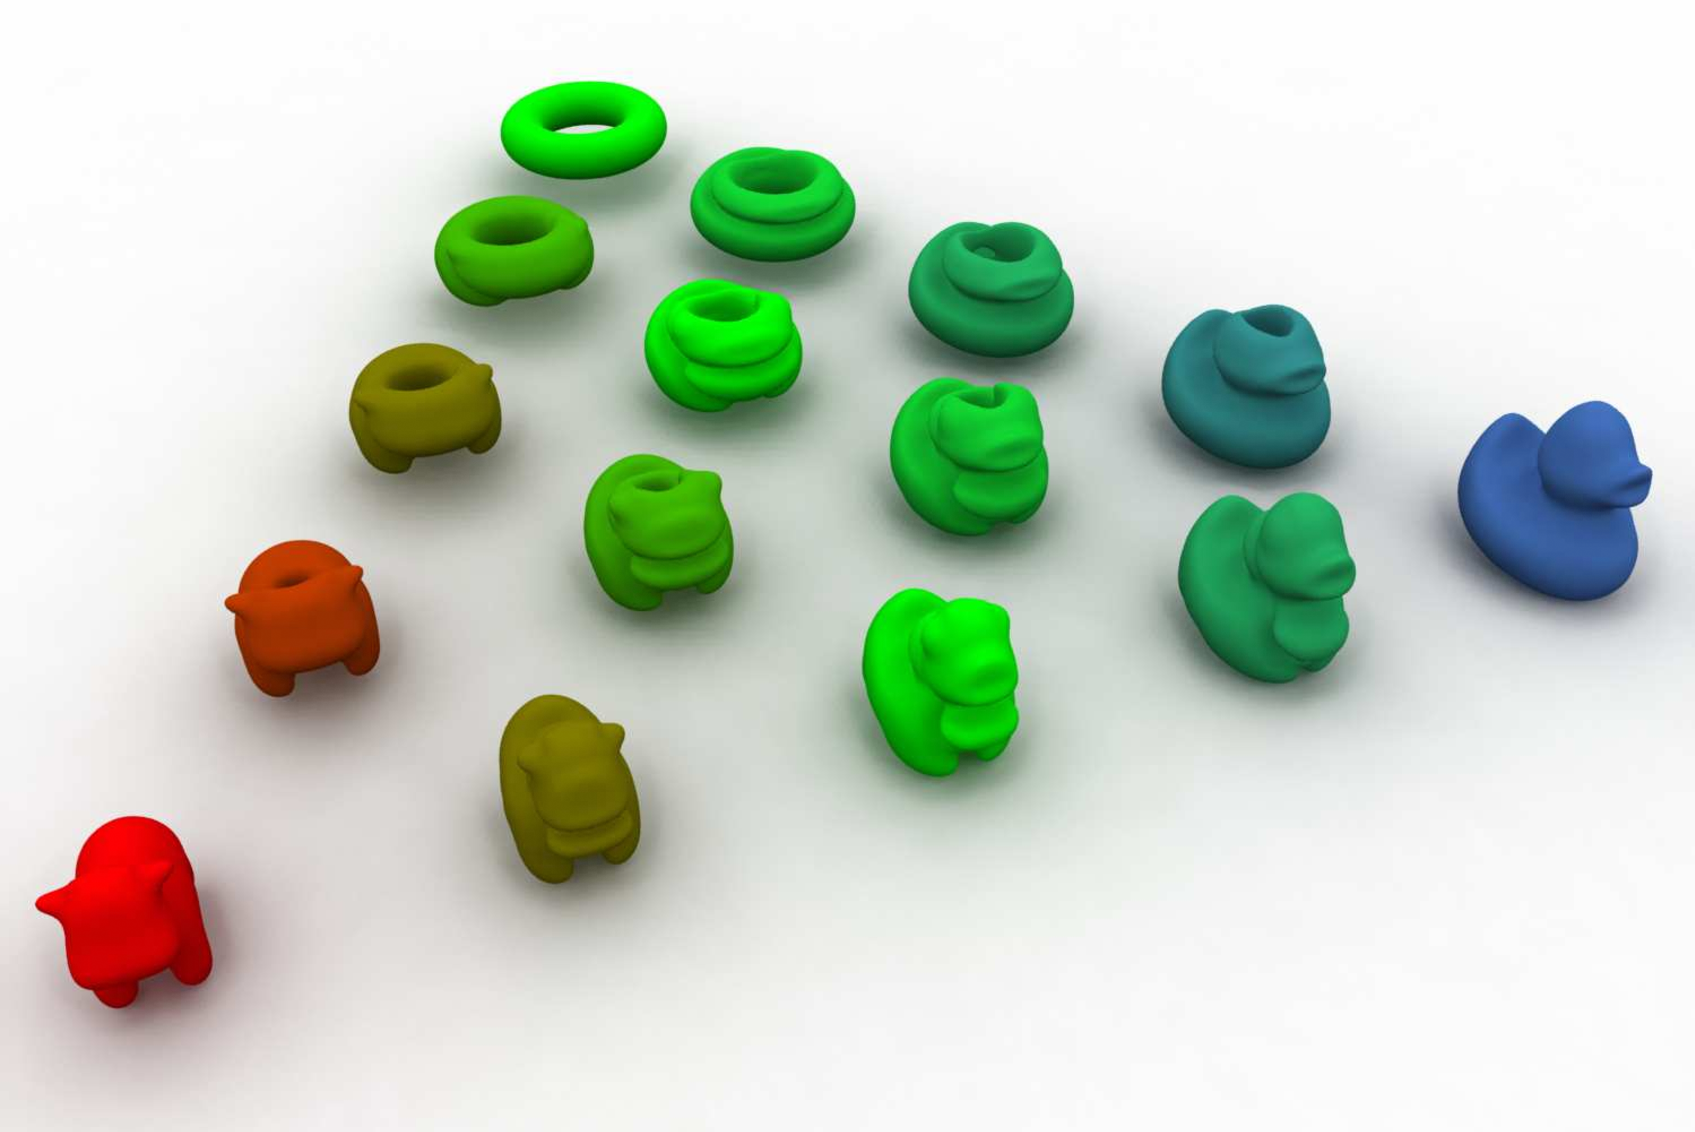
\includegraphics[width=.61\linewidth]{transport-hd/applis/shapes-3d}
\caption{Numerical barycentric interpolation of three-dimensional shapes represented by probability distributions. The three reference shapes occupy the vertices of the triangle; interior points correspond to different weights in~\eqref{eq-bary}.}\label{fig:barycenters}
\end{figure}

\subsection{Comparing texts}
Normalize word counts in a text to form a probability distribution. Transport can compare two such distributions using a cost that describes the dissimilarity between words, for example distances between word embeddings. The choice of this ground cost determines which substitutions are considered inexpensive; it may also be learned from a task~\cite{huang2016supervised}. Word histograms discard word order, so they cannot by themselves capture all grammatical or semantic distinctions.

\begin{figure}[htbp]\centering

\includegraphics[width=.40\linewidth]{transport-hd/applis/bag-word-1}\hspace{8mm}
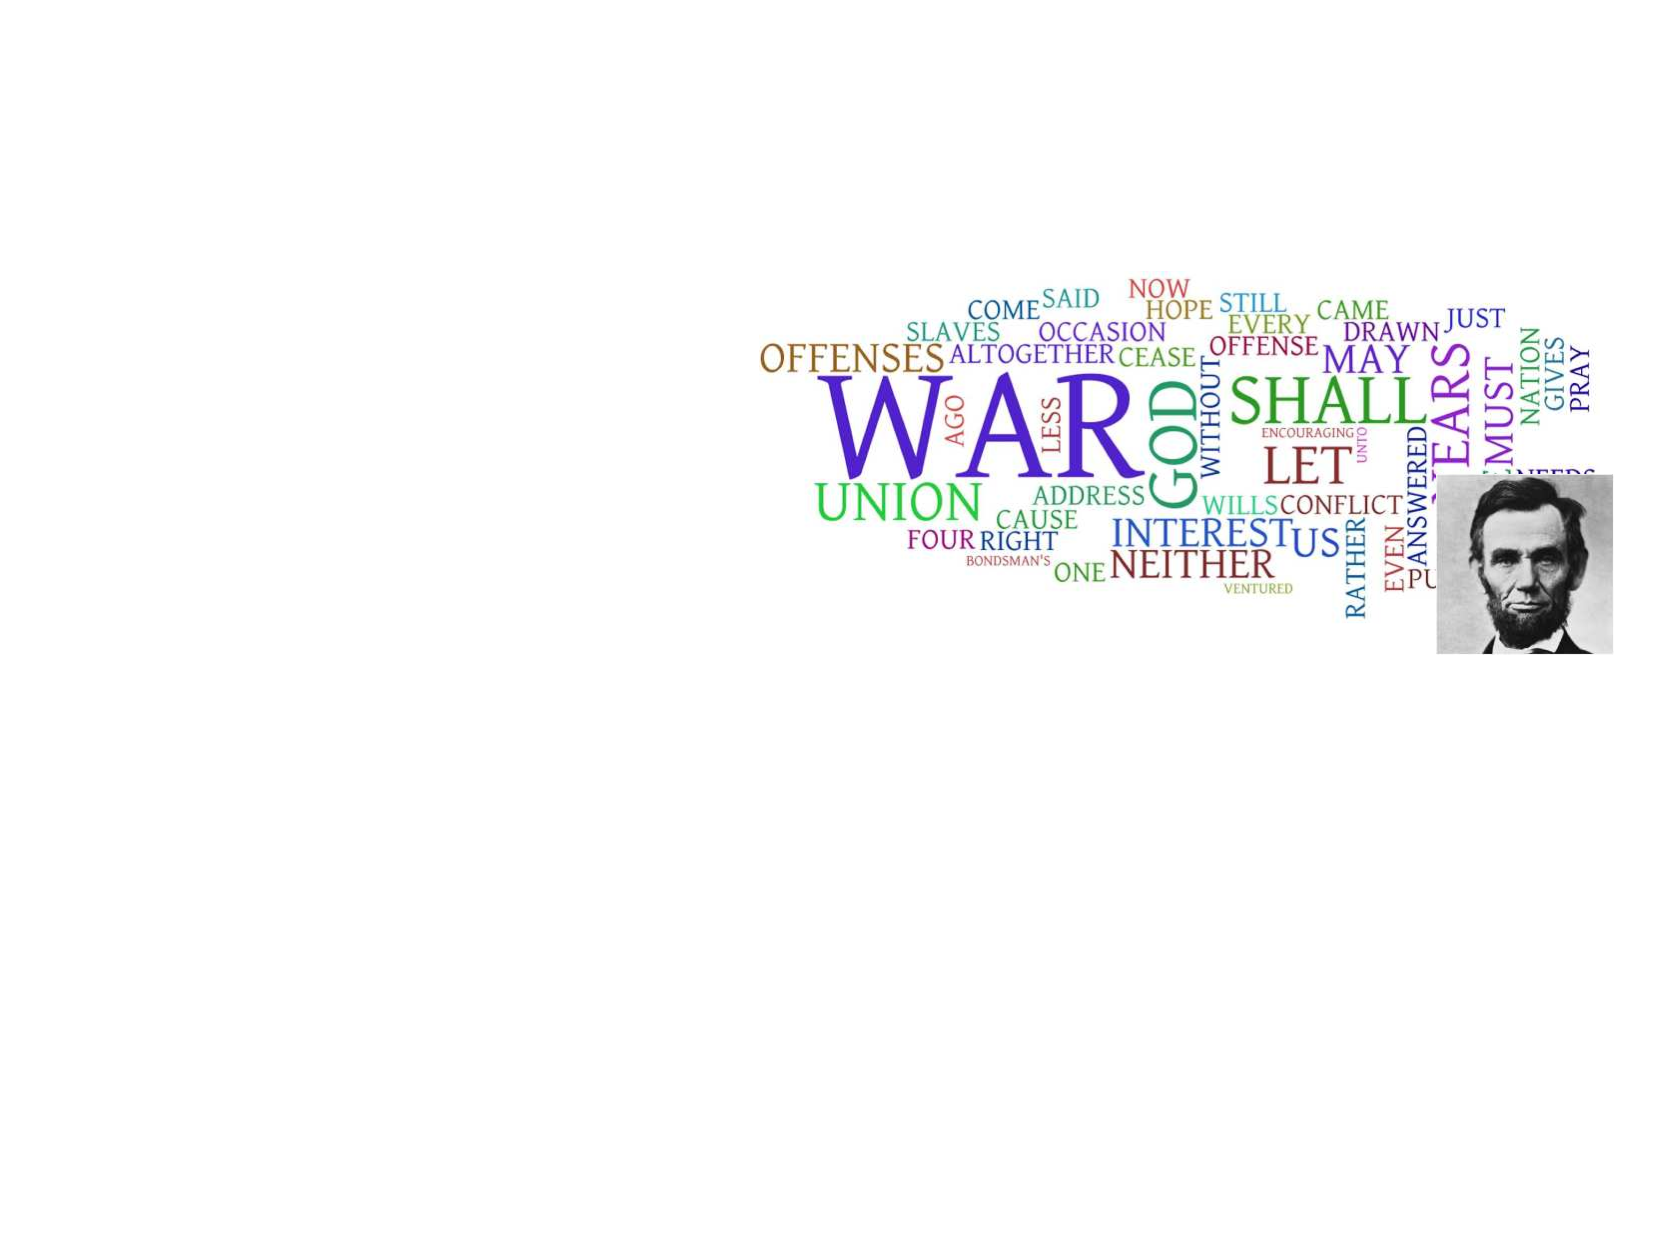
\includegraphics[width=.40\linewidth]{transport-hd/applis/bag-word-2}
\caption{Word clouds showing the most frequent words in two texts. Their sizes indicate relative frequencies; these are illustrations rather than a complete numerical histogram.}\label{fig:bagwords}
\end{figure}

\paragraph*{Further reading.}
For the theory, see~\cite{Villani03,SantambrogioBook}. Computational methods and applications are developed in~\cite{PeyreCuturi}. The companion course \href{https://www.gpeyre.com/ot4ml/}{Optimal Transport for Machine Learning (OT4ML)} offers another route into these ideas.

\ifdefined\StandaloneChapter
\paragraph*{Acknowledgements.}
I thank Vincent Beck, Gwenn Guichaoua, and Marie-Noëlle Peyré for their careful reading.
\fi
